\documentclass[tikz,border=2pt]{standalone}
\usepackage{amsmath,amssymb}
\usepackage{tikz}
\usetikzlibrary{arrows.meta}

\begin{document}
% R^2 = V1 (+) V2 for two distinct lines through the origin: each w splits in exactly one
% way as v1 + v2 with v1 in V1 and v2 in V2.
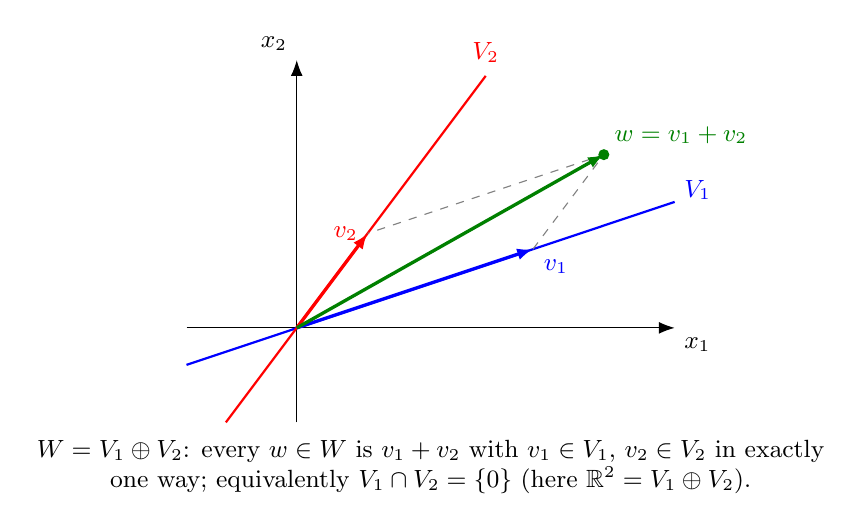
\begin{tikzpicture}[every node/.style={font=\small}, >={Latex[length=2mm]}]
	\draw[->] (-1.4,0) -- (4.8,0) node[below right] {$x_1$};
	\draw[->] (0,-1.2) -- (0,3.4) node[above left] {$x_2$};
	\draw[blue, thick] (-1.4,-0.47) -- (4.8,1.6);
	\node[blue, anchor=west] at (4.8,1.75) {$V_1$};
	\draw[red, thick] (-0.9,-1.2) -- (2.4,3.2);
	\node[red, anchor=south] at (2.4,3.25) {$V_2$};
	\draw[->, blue, very thick] (0,0) -- (3,1) node[below right, font=\small] {$v_1$};
	\draw[->, red, very thick] (0,0) -- (0.9,1.2) node[left, font=\small, inner sep=3pt] {$v_2$};
	\draw[dashed, gray] (3,1) -- (3.9,2.2) -- (0.9,1.2);
	\draw[->, green!50!black, very thick] (0,0) -- (3.9,2.2) node[above right] {$w=v_1+v_2$};
	\fill[green!50!black] (3.9,2.2) circle (2pt);
	\node[anchor=north, align=flush center, text width=10cm] at (1.7,-1.3) {$W=V_1\oplus V_2$: every $w\in W$ is $v_1+v_2$ with $v_1\in V_1$, $v_2\in V_2$ in exactly one way; equivalently $V_1\cap V_2=\{0\}$ (here $\mathbb{R}^2=V_1\oplus V_2$).};
\end{tikzpicture}
\end{document}
